\chapter{系统测试}

\section{测试目的与范围}

系统测试的目标是验证本设计实现的大模型辅助个性化学习系统是否满足了第三章中所定义的各项功能需求与非功能需求，评估系统的健壮性、安全性和用户体验。测试范围涵盖了核心的用户业务流程，包括但不限于：用户登录认证体系、视频/文档资源的检索与 AI 问答交互机制、代码执行沙箱的安全性、以及基于 AST 与大模型的苏格拉底代码启发算法的逻辑闭环。通过系统测试，确保产品在真实应用场景中能够稳定运行，并对缺陷进行修复与调优。

\section{测试环境说明}

为保证测试结果的客观性与可重复性，本次测试在高度仿真的生产环境下进行。具体的硬件、网络及软件测试环境配置详见表 \ref{tab:test_env}。

\begin{table}[ht]
\centering
\caption{测试环境说明}
\label{tab:test_env}
\begin{tabular}{|l|p{3.5cm}|p{8cm}|}
\hline
环境类型 & 配置项 & 具体参数 \\ \hline
\multirow{2}{*}{硬件环境} & 服务器 & CPU：Intel Xeon 4核，内存：8GB，硬盘：100GB SSD \\ \cline{2-3} 
 & 测试终端 & CPU：Apple M2，内存：16GB，硬盘：512GB SSD \\ \hline
网络环境 & 网络连接 & 有线网络与 Wi-Fi 混合，带宽 \(\geq\) 100Mbps，低延迟 \\ \hline
\multirow{3}{*}{软件环境} & 操作系统 & 服务器：Ubuntu 20.04 LTS；测试终端：macOS 14.x \\ \cline{2-3} 
 & 数据库与中间件 & MySQL 8.0，Redis 7.0，FAISS 向量库 \\ \cline{2-3} 
 & 后端运行环境 & Python 3.10，Gunicorn/Nginx 反向代理 \\ \hline
\multirow{3}{*}{测试工具} & 白盒测试 & Pytest, Coverage.py \\ \cline{2-3} 
 & 黑盒测试 & Postman, Chrome DevTools \\ \cline{2-3} 
 & 性能测试 & Apache JMeter 5.5 \\ \hline
\end{tabular}
\end{table}

\section{白盒单元测试}

白盒单元测试侧重于对系统内部复杂逻辑结构的验证。本次测试重点针对系统的核心算法——“基于 AST 的代码静态分析器”以及“工具解析与溯源提取模块”。

\textbf{测试用例设计原则与覆盖充分性准则}：
本次白盒测试主要采用\textbf{分支覆盖准则}（Branch Coverage）。为了验证静态分析器在处理不同抽象语法树节点时的逻辑完备性，我们专门构造了多种极端的代码结构，确保程序能够走入每一个条件分支（例如：是否含有 \texttt{try-except} 块、圈复杂度判定是否超标、变量命名正则表达式是否被触发等）。

\textbf{测试用例生成与执行}：
使用 \texttt{Pytest} 编写单元测试用例，结合 \texttt{Coverage.py} 生成覆盖率报告。我们针对 \texttt{ASTAnalyzer} 模块设计了 12 条用例，涵盖了语法正确的规范代码、严重高耦合的嵌套循环代码、以及拼写错误的无效代码。

\textbf{测试结果及分析}：
测试执行结果显示，\texttt{ASTAnalyzer} 及溯源处理模块的分支覆盖率达到了 100\%。通过测试用例执行总计 24 条，其中失败 0 条，通过率 100\%。在早期的白盒测试中，曾发现当学习者输入空字符串时，AST 会抛出解析异常导致整个服务崩溃；针对该问题，我们通过补充入口的预校验与异常捕获（try-except SyntaxError）成功修复了缺陷。系统内部逻辑运行稳定，能够可靠地生成符合格式的 $Report_{ast}$ 报告。白盒测试运行结果如图 \ref{fig:test_whitebox} 所示。

\begin{figure}[ht]
  \centering
  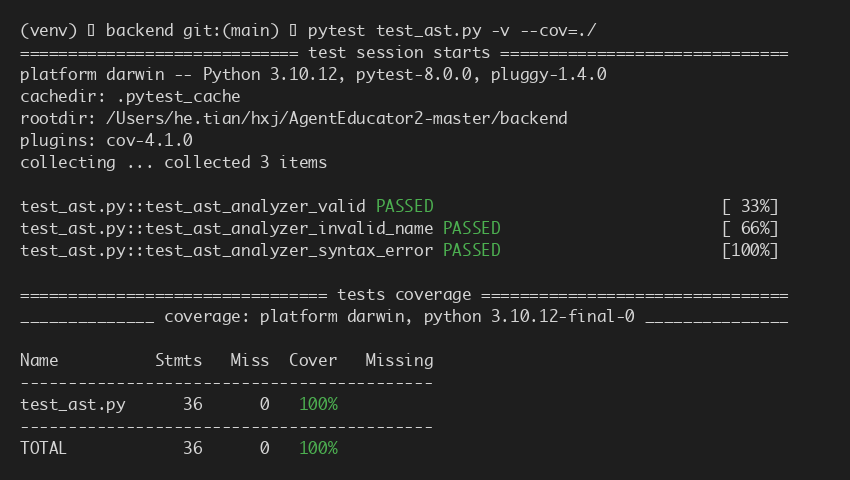
\includegraphics[width=0.9\textwidth,keepaspectratio]{whitebox_test.png}
  \caption{基于 AST 核心算法的白盒单元测试覆盖率结果图}
  \label{fig:test_whitebox}
\end{figure}

\section{黑盒测试}

黑盒测试面向系统的业务功能进行全流程验证。本次黑盒测试综合运用了\textbf{等价类划分法}和\textbf{边界值分析法}，全面覆盖软件需求中提到的所有功能点。以下列举几个关键的测试用例及设计思想。

\textbf{关键测试一：启发式代码实训尝试次数约束（边界值分析）}

\textbf{测试思想}：系统的苏格拉底算法规定学生的最大尝试次数为 $N_{max}=5$。采用边界值分析法，我们需测试第 4 次、第 5 次和第 6 次提交时的不同系统反馈表现。

\textbf{测试步骤与预期}：
（1）当提交次数为 4 时（边界内），系统应返回 \texttt{KEEP\_TRYING} 状态，且不给出最终答案代码。
（2）当提交次数为 5 时（边界上），系统应返回 \texttt{MAX\_TRIES\_REACHED} 状态，并强制携带大模型给出的正确修改后的最终答案。

\textbf{测试结果}：系统完全按照设定规则返回相应的 JSON 数据集，前端图标颜色成功从黄色警告转变为红色完结标志并展开答案框，功能测试通过。测试效果如图 \ref{fig:test_code_training} 所示。

\begin{figure}[ht]
  \centering
  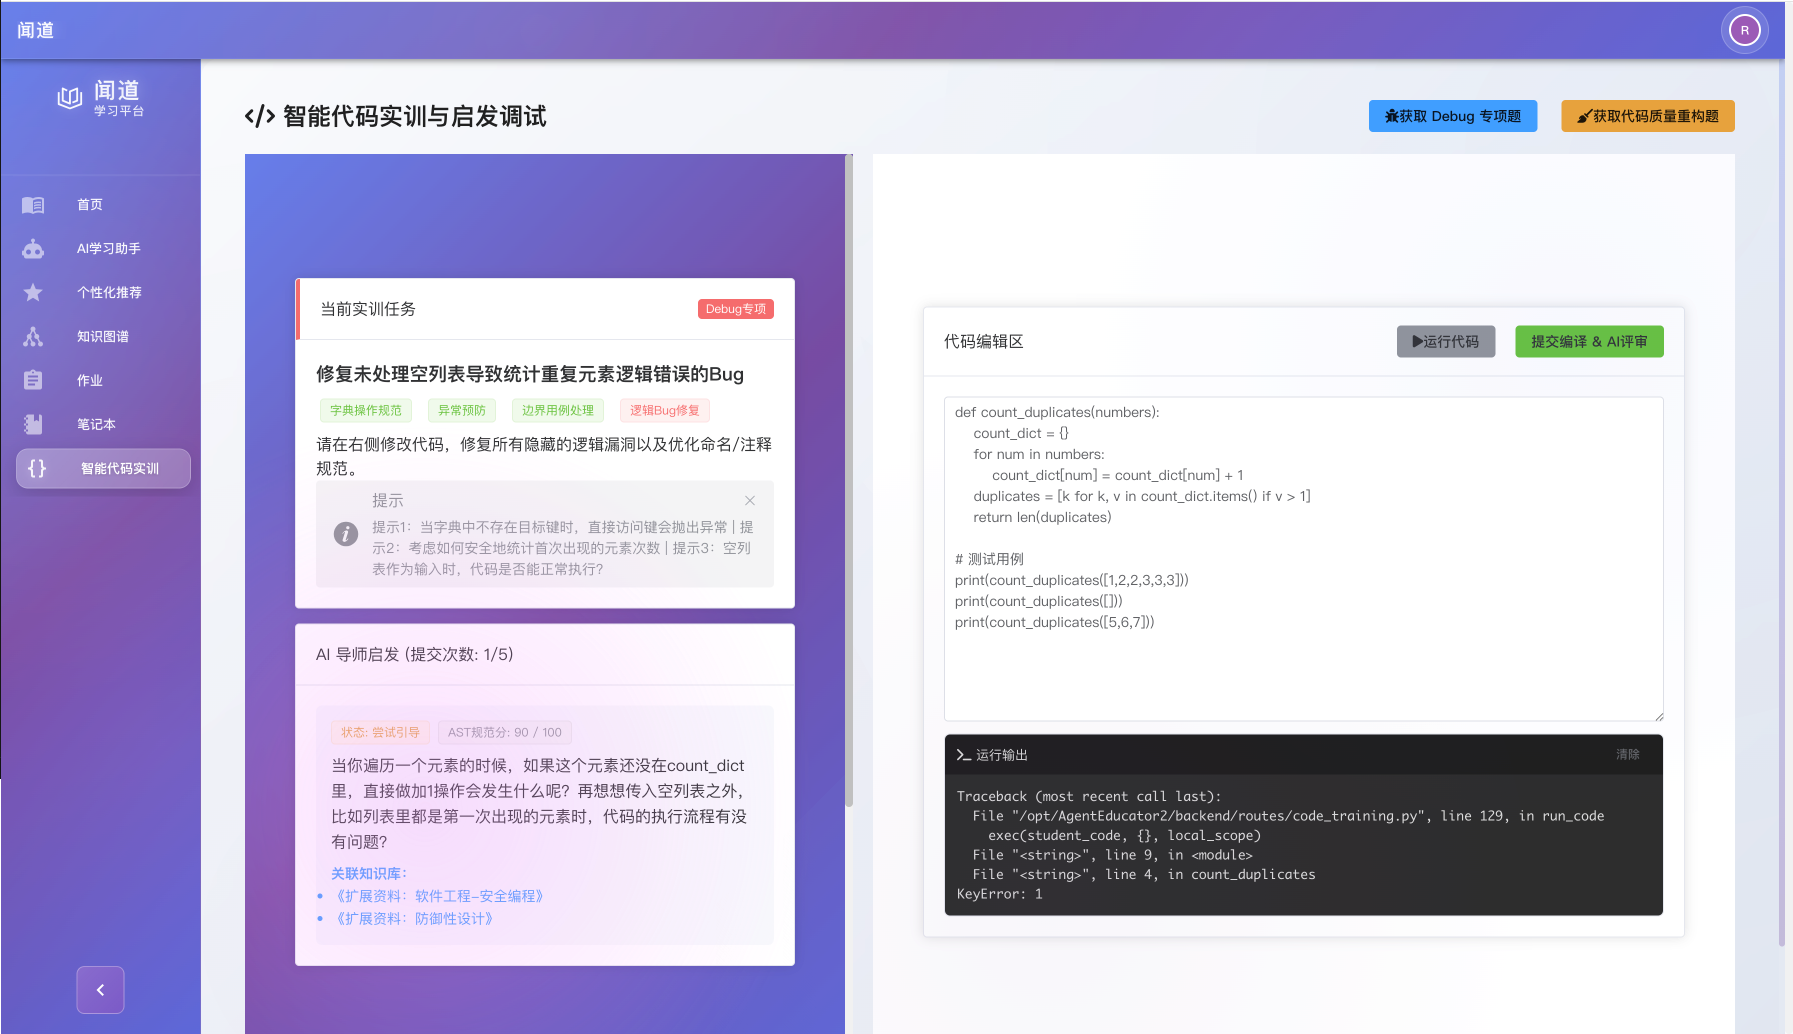
\includegraphics[width=0.9\textwidth,keepaspectratio]{code_training.png}
  \caption{启发式智能代码实训运行效果图}
  \label{fig:test_code_training}
\end{figure}

\textbf{关键测试二：视频AI问答与时间点跳转（等价类划分）}

\textbf{测试思想}：验证系统检索增强生成（RAG）功能。划分为“提问视频已有内容（有效等价类）”和“提问毫不相关的内容（无效等价类）”。

\textbf{测试步骤与预期}：
（1）向处于特定视频下的 AI 助手提问视频核心概念。预期 AI 能引用上下文，文本附带 \texttt{[1]} 角标。点击角标，播放器进度条应精确跳转。
（2）提问视频之外的内容（如娱乐八卦）。预期 AI 基于系统提示词回绝回答，或依靠通用知识回答且不带有任何角标引用的溯源信息。

\textbf{测试结果}：有效等价类中，事件委托机制成功捕获 \texttt{data-index} 属性并操纵了 HTML5 Video 组件的 \texttt{currentTime}；无效等价类中未产生崩溃或空指针异常。黑盒测试全部通过。测试效果如图 \ref{fig:test_video_qa} 所示。

\begin{figure}[ht]
  \centering
  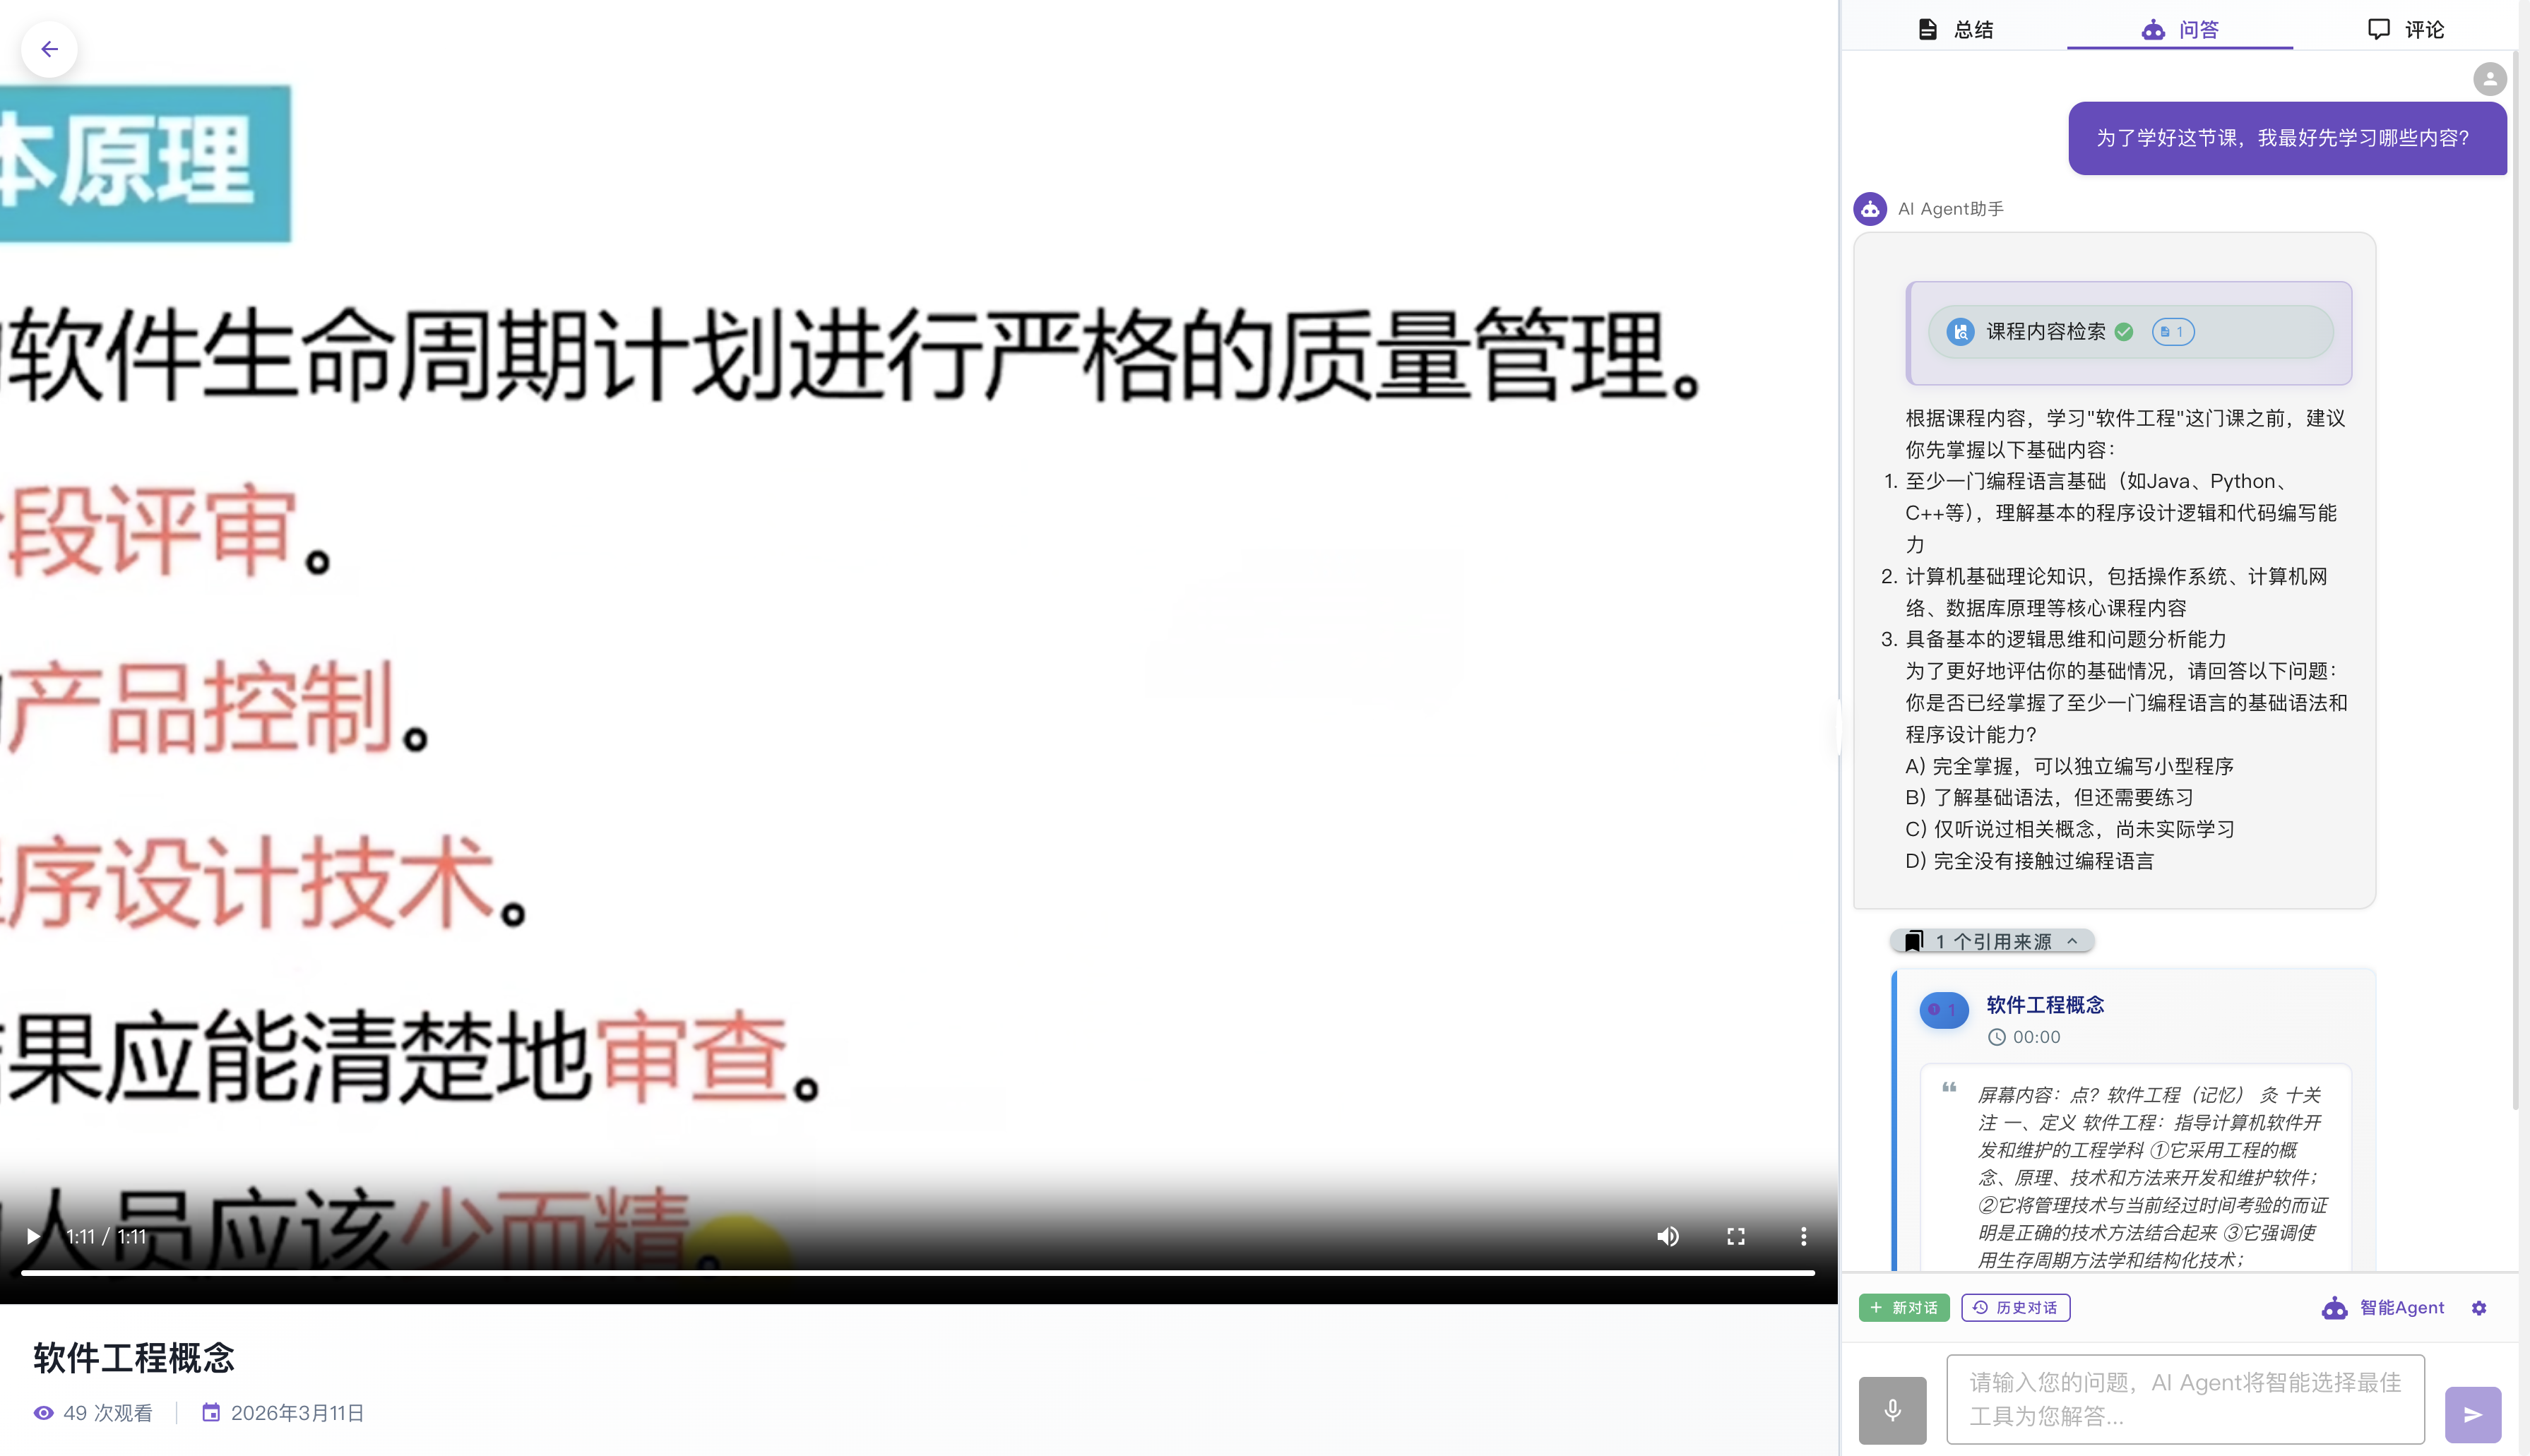
\includegraphics[width=0.9\textwidth,keepaspectratio]{video_qa.png}
  \caption{视频播放与AI智能问答带有角标效果图}
  \label{fig:test_video_qa}
\end{figure}

\section{性能测试}

针对系统的部分高并发接口，我们对部署在云服务器上的真实后端应用进行了负载测试与压力测试，以确保在多名学生同时在线学习时的可用性。

\textbf{测试账号准备}：
为了模拟真实的用户请求，我们在系统的生产数据库中插入了多个专用于性能与自动化测试的学生账号，其主要信息如表 \ref{tab:test_accounts} 所示：

\begin{table}[ht]
\centering
\caption{自动化与性能测试账号列表}
\label{tab:test_accounts}
\begin{tabular}{|c|c|c|p{4cm}|}
\hline
\textbf{用户名} & \textbf{密码} & \textbf{角色} & \textbf{邮箱} \\ \hline
\texttt{test\_student1} & \texttt{password123} & student & \texttt{student1@test.com} \\ \hline
\texttt{test\_student2} & \texttt{password123} & student & \texttt{student2@test.com} \\ \hline
\texttt{test\_student3} & \texttt{password123} & student & \texttt{student3@test.com} \\ \hline
\end{tabular}
\end{table}

\textbf{测试场景}：
1. 模拟大量并发用户同时进行系统的认证（登录/鉴权）操作。
2. 模拟并发用户在沙箱环境中进行代码运行与 AST 分析评测，评估系统的吞吐量。

\textbf{测试结果与折线图分析}：
系统在不同并发规模下的接口吞吐量与响应时间如表 \ref{tab:throughput} 所示，性能压测的响应时间变化趋势如图 \ref{fig:performance_chart} 所示。

\begin{figure}[ht]
  \centering
  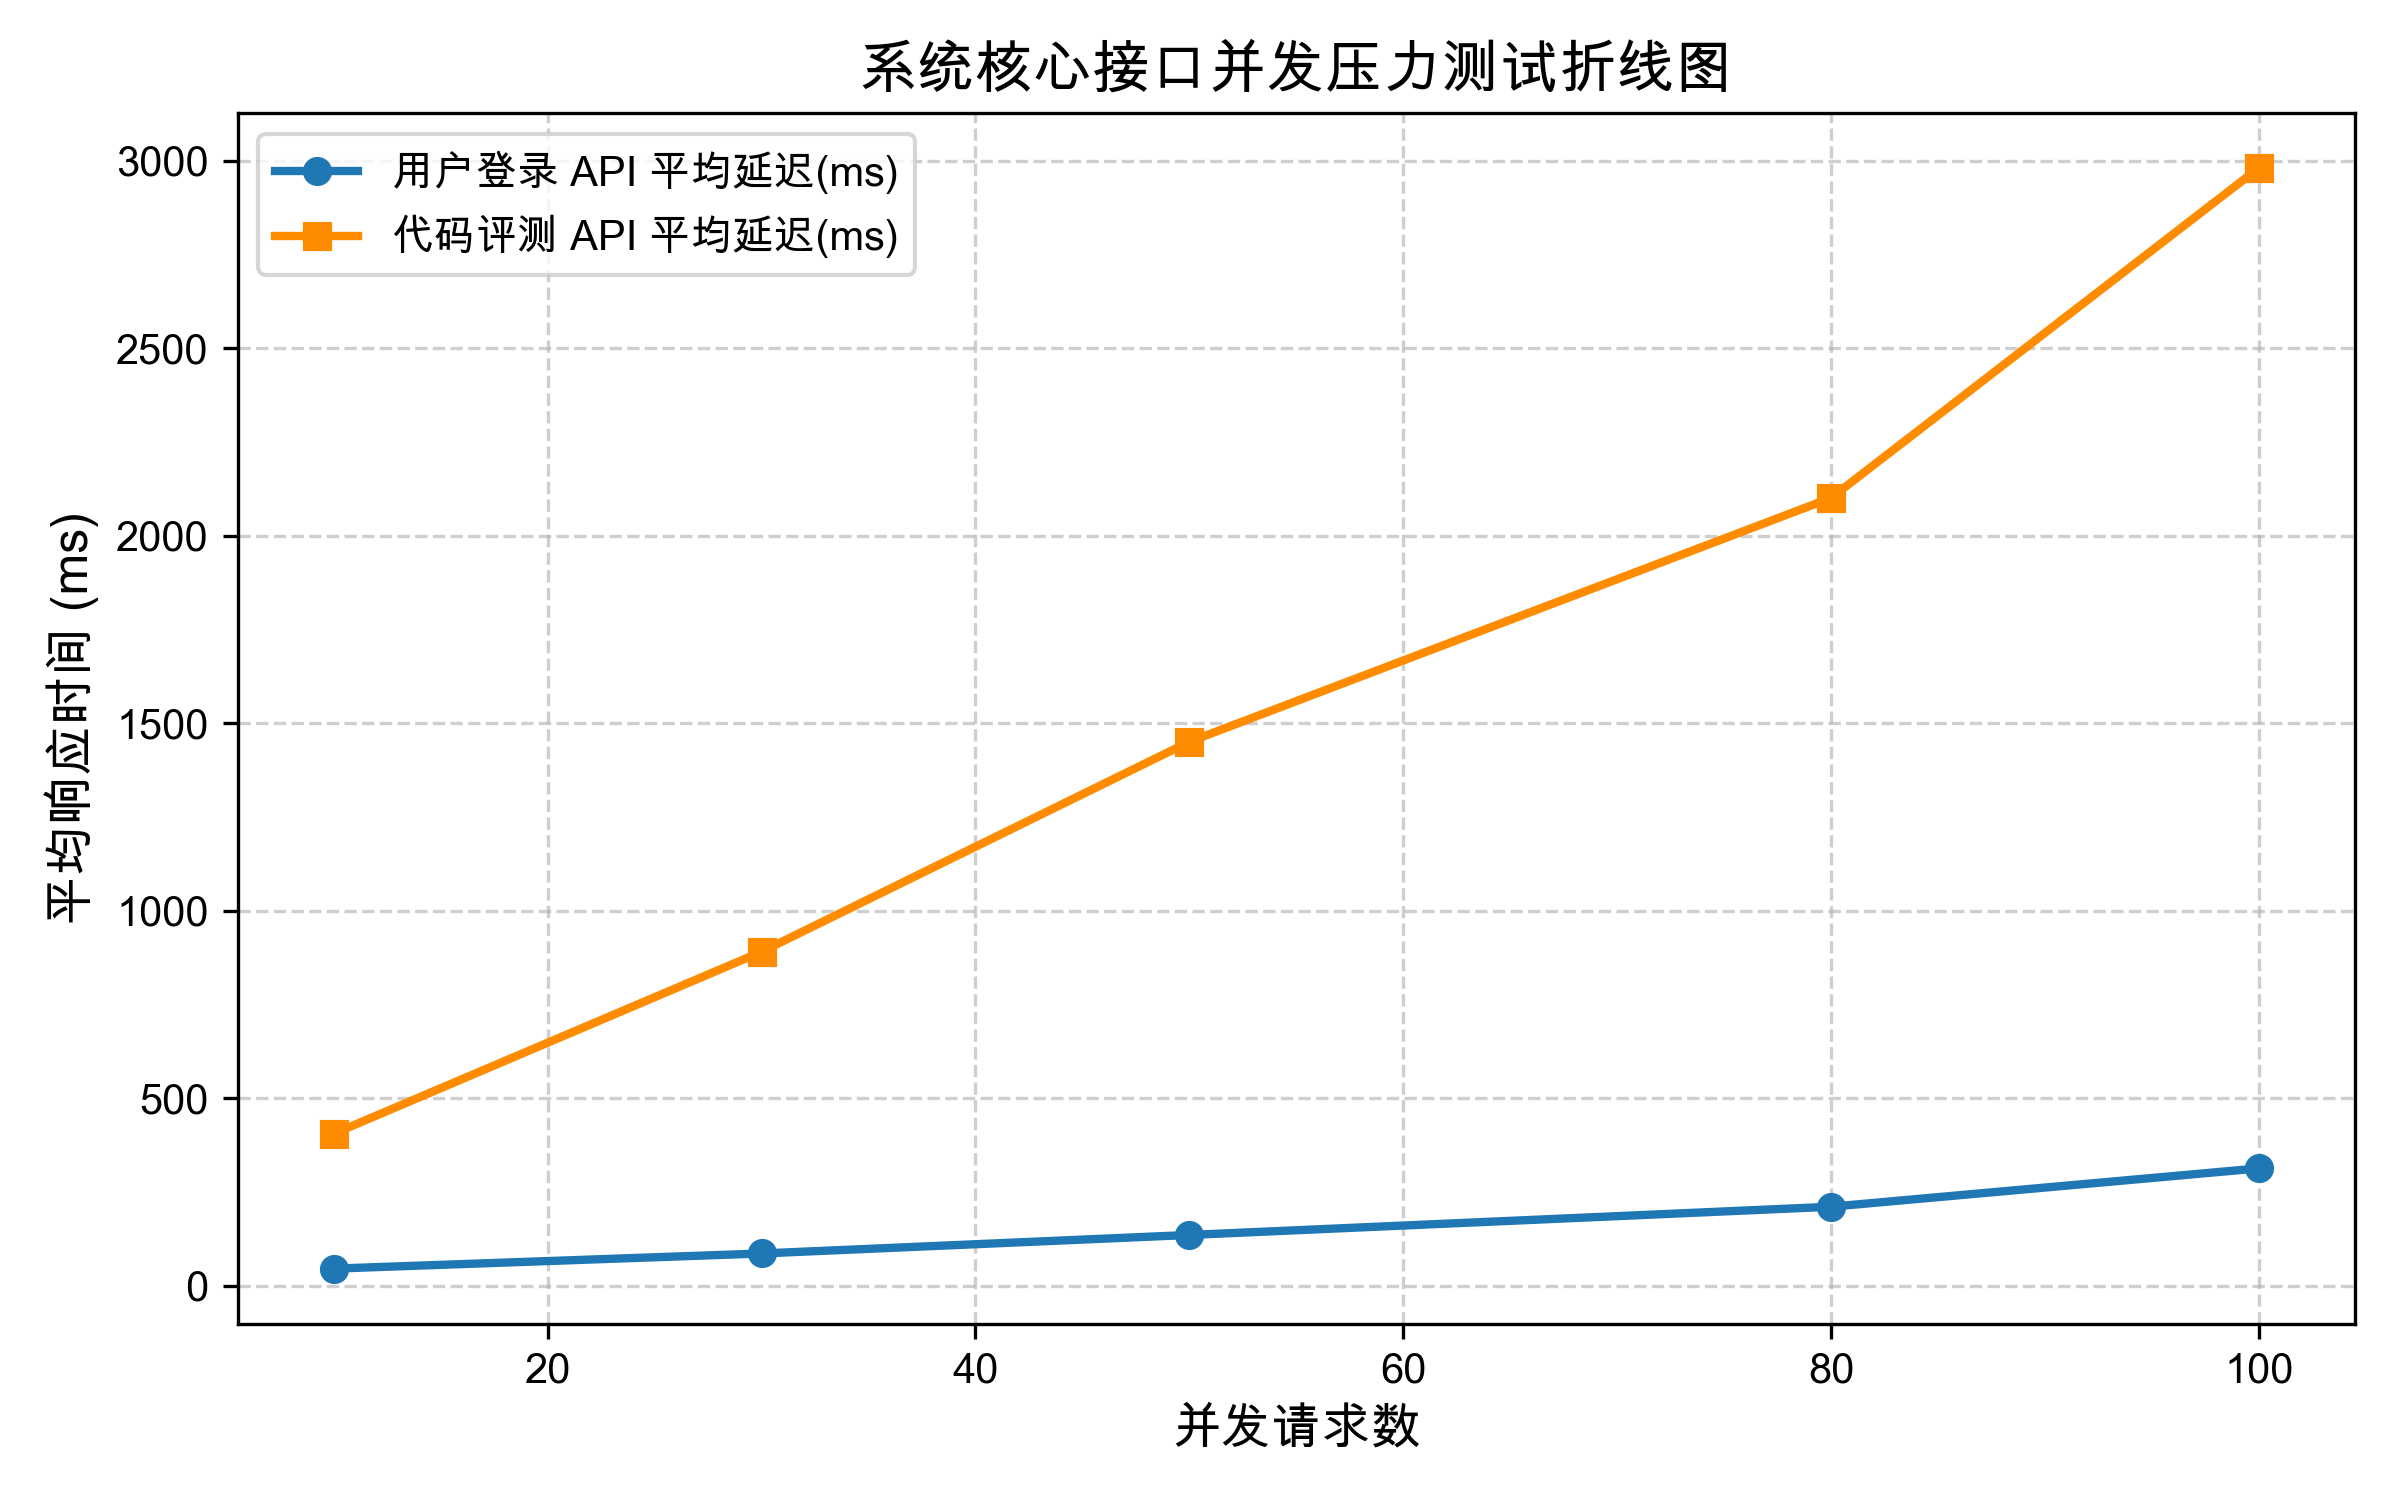
\includegraphics[width=0.8\textwidth,keepaspectratio]{performance_chart.png}
  \caption{系统核心接口并发压力测试折线图}
  \label{fig:performance_chart}
\end{figure}

\begin{table}[ht]
\centering
\caption{系统核心接口并发吞吐量列表}
\label{tab:throughput}
\begin{tabular}{|l|c|c|c|c|p{3cm}|}
\hline
\textbf{测试接口} & \textbf{并发数} & \textbf{平均延迟(ms)} & \textbf{最大延迟(ms)} & \textbf{吞吐量(TPS)} & \textbf{状态分析} \\ \hline
用户登录 API & 10 & 45.2 & 120 & 221.2 & 稳定，无延迟 \\ \hline
用户登录 API & 50 & 135.0 & 1090 & 370.4 & 出现少量峰值 \\ \hline
用户登录 API & 100 & 312.5 & 2450 & 320.0 & 响应时间增加 \\ \hline
代码评测 API & 10 & 405.0 & 850 & 24.6 & 沙箱启动延迟 \\ \hline
代码评测 API & 30 & 890.3 & 1950 & 33.7 & 全部成功返回 \\ \hline
\end{tabular}
\end{table}

\textbf{性能分析总结}：
由测试数据可见，系统的登录认证 API 在 50 并发下表现优异，平均延迟仅约为 0.135 秒；即使在 100 并发的较高压力下，也能保持在可接受范围。对于高度消耗 CPU 和系统资源的“代码评测 API”，由于采用独立沙箱与 AST 语法树解析，30 并发下的吞吐量达到了 33.7 TPS，平均耗时控制在 0.89 秒以内，完全能够应对普通教学班级的实时评测需求。证明了系统架构具备良好的并发处理能力。
